% !TeX root = ../main.tex

\chapter{绪论}

\section{研究背景和意义}

随着全球科技竞争的加剧,信息技术自主可控已成为国家战略的重要组成部分。龙芯作为国产处理器的代表,其生态系统的完善和应用推广对打破国外技术垄断、实现核心技术自主化具有重要意义。
然而,目前龙芯平台主要集中于桌面和服务器领域,在移动设备领域的应用仍处于空白或起步阶段。因此,基于龙芯平台开发移动设备相关技术,不仅是对国产处理器生态的扩展,
更是对国家信息技术自主化战略的重要支持。

而相应的,Android 系统作为全球最广泛使用的移动操作系统之一,其意义和重要性不言而喻。
根据 statcounter 的数据,2023 年11月至2024年11月全球智能手机市场中,Android 系统的市场份额均超过 70\%\cite{MobileMarket}。
这意味着大量的用户依赖于 Android 平台进行日常操作和娱乐。
\begin{figure}[h]
    \centering
    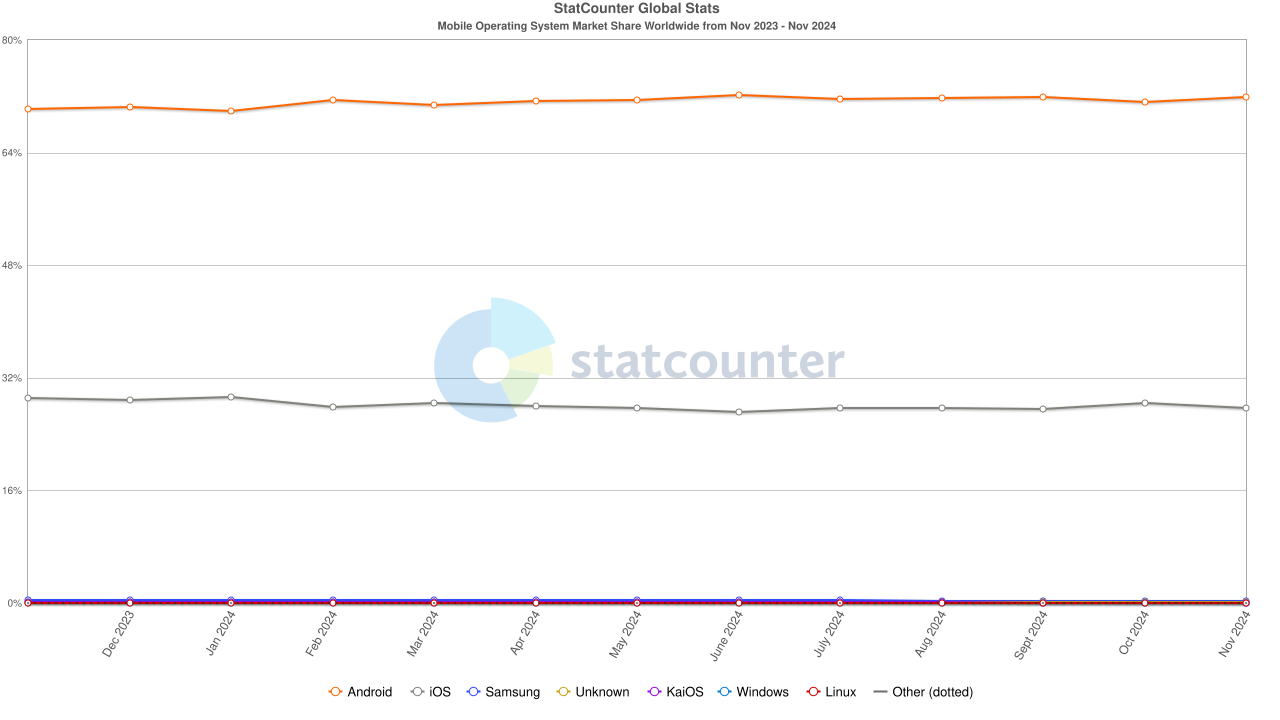
\includegraphics[width=0.8\textwidth]{2024全球智能手机市场占有率统计.png}
    \caption{2024全球智能手机操作系统市场占有率统计}\cite{MobileMarket}
  \end{figure}
Android作为Google公司开发的开源操作系统,其在国内市场也有广泛的应用领域,滋养了移动端设备的蓬勃发展。但是中美科技战的背景下,
高端移动设备的芯片进口受到限制,产业发展受制于人。龙芯作为国产自主芯片的领头羊,于2021年推出了自主指令集Loongson Architecture(LoongArch)\cite{Loongarch},
涵盖基础架构、虚拟化、向量指令等多个部分。由于龙芯目前多专注于桌面、服务器以及嵌入式领域,新型的LoongArch架构也尚未支持主流的安卓或鸿蒙等开源操作系统,
因此亟待移动端基础软件的支持以及软件生态的建设。将安卓移植到龙芯指令集上不仅有利于丰富完善龙芯的软件生态,而且会为后续的移动端国产化替代提供一个探索性的方案,
是非常有意义的。

Android 的图形系统作为Android系统最基础最重要的模块之一,图形系统的正确运行与否直接导致zygote(所有Android应用进程的起点)进行能否顺利创建。
而同时,Android图形系统又是一个极为复杂的系统,其复杂性体现在其多层架构中,包括应用层、框架层、硬件抽象层(HAL)及底层驱动。
这种多层结构使得开发者能够灵活地利用不同的图形 API,在设计上具有高度的灵活性和可扩展性,但却极大的增加了安卓框架本身的复杂性,使得在实际应用中仍面临诸多挑战。
例如,不同设备的硬件差异使得图形性能的优化变得复杂。这使得开发者需要针对不同设备进行优化,以确保应用在各种硬件上的流畅运行。
此外,Android 的多任务处理机制可能导致图形渲染时的资源竞争,进而影响应用的响应速度和帧率。这一问题在资源密集型应用中尤为明显,如大型游戏或复杂的图形应用。
研究表明,游戏应用中的帧率波动会直接影响用户的留存率,帧率是影响用户满意度的关键因素\cite{claypool2006effects}。

通过对图形系统的研究和优化,可以提高应用程序的图形渲染效率,加快界面的响应速度,降低卡顿现象的发生频率。此外
一个稳定的图形栈可以减少应用程序崩溃和系统崩溃的可能性,提高系统的稳定性和可靠性,保障
用户数据的安全性;优化应用程序的图形渲染流程,提高应用程序的性能表现,减少资源占用,降
低功耗消耗,从而提升开发效率和节约开发成本。因此,对 Android 图形栈的研究具有重要的理论和实际意义。

本课题旨在探索利用基于龙芯平台,实现一个使用龙芯国产CPU和GPU的安卓图形系统设计方案,解决龙芯安卓图形系统中一系列基础依赖库或软件等问题,
为后续的一系列基于安卓系统的开发打下基础,推动安卓项目的顺利进行。

\section{国内外研究现状}

\subsection{安卓生态显卡驱动发展路径}
安卓系统上的显卡驱动技术发展可归纳为四大核心阶段,其演进主线从基础图形支持到性能与生态优化,最终向智能化和跨平台协同迈进:

\subsubsection{基础图形框架搭建(Android 2.x-4.x时代)}

此阶段以构建基础图形渲染能力为核心目标,通过OpenGL ES 1.x/2.0接口实现移动端图形管线标准化\cite{opengles}。
硬件抽象层(HAL)作为GPU与Android显示合成服务(SurfaceFlinger)之间的桥梁,负责将用户态图形API调用转化为底层GPU指令,
支持2D界面绘制与早期3D游戏渲染。然而,由于GPU厂商(如高通Adreno、Arm Mali\cite{mali}、Imagination PowerVR)硬件架构差异显著,
驱动实现高度碎片化,导致开发者需针对不同硬件编写优化代码。Google通过兼容性测试套件(CTS)规范驱动接口行为,
但实际性能优化仍依赖厂商自行实现。此阶段的技术瓶颈集中在显存管理效率不足、多线程渲染支持缺失以及功耗控制机制原始,难以满足复杂应用场景需求。

\subsubsection{性能优化与标准化(Android 5.x-8.x时代)​}

随着移动设备屏幕分辨率提升与高帧率游戏需求激增,驱动技术转向深度性能优化与生态标准化。
Google推出Project Butter项目,在驱动层引入垂直同步(VSYNC)与三重缓冲机制,通过动态调整GPU渲染节奏降低画面撕裂与卡顿现象\cite{GoogleIO2012}。
Android 7.0正式集成Vulkan API,其低开销设计(Explicit API)与多线程命令提交特性显著降低CPU负载,
驱动需重构指令调度器以支持并行化渲染管线(如Mali Midgard架构驱动实现多核Shader Core负载均衡)\cite{vulkan}。
同期,GPU Profiling工具链(如Systrace、GPU渲染模式分析器)的完善迫使驱动层暴露硬件性能计数器(如像素填充率、纹理采样周期),
辅助开发者定位渲染瓶颈。此阶段的技术突破在于通过API与工具链标准化削弱生态碎片化,
同时借助硬件架构升级(如Adreno 500系列引入统一着色器架构\cite{adreno})实现能效比跃升。

\subsubsection{异构计算与驱动模块化(Android 9.x-12时代)​}

移动GPU从专用图形处理器向通用计算加速器转型,驱动技术重点扩展至异构计算支持与架构解耦。
驱动层集成OpenCL与Vulkan Compute后端,使GPU能够加速机器学习推理(如TensorFlow Lite模型部署\cite{tflite_gpu})、
物理模拟等非图形任务,高通Adreno 600系列驱动甚至通过AI协处理器(Hexagon DSP)实现异构任务卸载。
Project Treble项目重构Android底层架构\cite{treble},通过硬件接口定义语言(HIDL)将GPU驱动封装为独立模块\cite{hidl},
支持通过Google Play系统更新独立推送驱动补丁。为适配90Hz/120Hz高刷新率屏幕,驱动引入自适应刷新率(VRR)与异步时间扭曲(ATW)技术,
优化触控输入到GPU渲染的端到端延迟(降至10ms以内),并采用分块延迟渲染(TBDR)架构降低带宽占用。
此阶段的技术重心在于打破传统图形边界,构建驱动与AI框架、显示子系统及外设输入的协同生态。

\subsubsection{开源生态与前沿技术融合(Android 13+及未来)​​}

当前阶段以开源化、云端协同与实时图形技术突破为标志。Arm主导的Panfrost项目\cite{panfrost}开源Mali GPU驱动代码,推动开源图形栈(Mesa 3D)适配安卓系统\cite{mesa},
降低厂商定制成本并提升安全审计透明度\cite{panfrost}。硬件光线追踪单元的引入要求驱动支持Vulkan Ray Tracing扩展\cite{vulkan_raytracing},
实现移动端动态全局光照(如UE5 Lumen技术简化版)与软阴影渲染加速。云游戏与元宇宙需求催生虚拟化GPU驱动架构,
Android Virtualization Framework支持多实例渲染上下文隔离,并通过AV1编解码硬件卸载降低云端流媒体传输延迟\cite{avf}。
AI技术进一步渗透至驱动层,利用机器学习模型预测着色器编译热点(如Shader Caching AI),动态优化资源分配策略,
并结合Android动态性能框架(ADPF)实现能效最优调度。未来技术路线将聚焦于纳米级几何渲染(Nanite-like管线优化)、
实时路径追踪与端边云协同渲染协议(如Google Stadia演进技术),驱动角色从硬件适配层升级为跨域算力调度中枢。

\subsection{与非ARM架构的兼容}
由于安卓图形系统较为重要,因此有部分开源项目以及学者提供了一些方案,以期同时兼顾兼容性和高效性。以下是一些方案的介绍。
张超等实现了SurfaceFlinger在桌面Linux的X Window环境下运行。其主要方法是通过替换gralloc硬件模块使用Linux上的窗口引擎,
也就是使用软件渲染的方式将SurfaceFlinger合成的图像写入共享内存,
再由一个桌面图形程序输出画面。该方法的不足是使用软件渲染而没有调用GPU实现硬件加速,造成占用大量CPU时间,并且画面输出过程需要不断调用IPC,
在处理3D图形时只有个位数的帧数,性能较为低下\cite{张超2012Android}。

\begin{figure}[H]
  \centering
  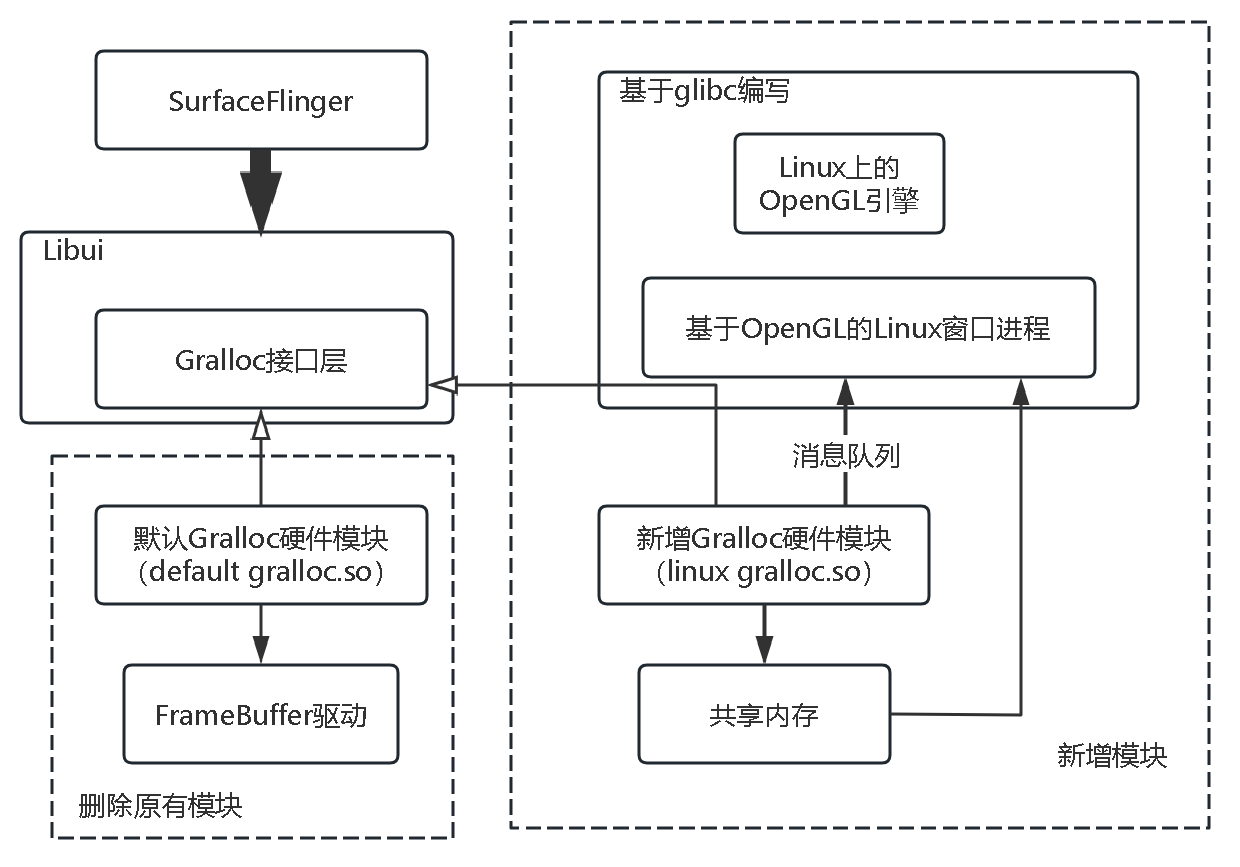
\includegraphics[width=0.6\textwidth]{Android图形系统向桌面Linux的移植.pdf}
  \caption{Android图形系统向桌面Linux的移植\cite{张超2012Android}}
\end{figure}

Android X86项目在X86架构的PC上运行Android系统,该项目使用Mesa\cite{mesa}的OpenGL ES实现,并基于DRM\cite{DRM}和GEM\cite{GEM}实现了gralloc.drm模块,
成功运行了可在X86架构下运行硬件加速的SurfaceFLinger\cite{AndroidX86}。在此基础上,江帆等提出了一种可以在X Window系统下运行Android SurfaceFlinger的方案,
具体是使用Mesa作为OpenGL ES实现并使Mesa EGL兼容Android的本地窗口,实现了能够GPU硬件加速的图形合成过程,另外使用DRI2拓展避免了图像缓存由独显到系统内存的拷贝过程\cite{XTYY201710015}。

\begin{figure}[H]
  \centering
  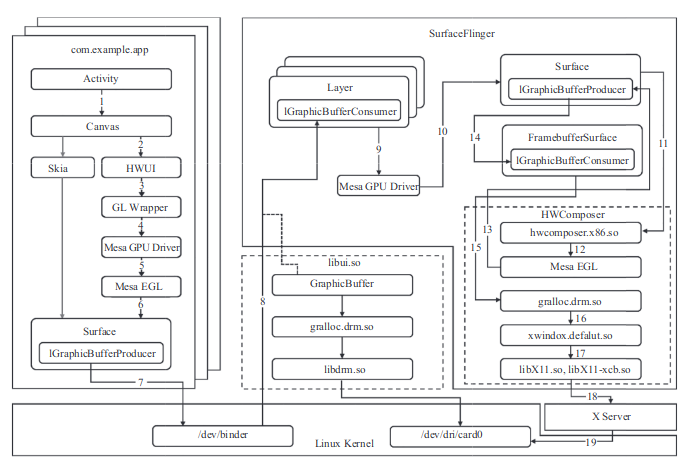
\includegraphics[width=0.8\textwidth]{SurfaceFlinger移植X环境架构.png}
  \caption{SurfaceFlinger移植X环境架构\cite{XTYY201710015}}
\end{figure}

李全刚设计了一种新的图形系统框架,其参考了安卓图形系统的设计思想,采用分层的架构实现,包括系统平台层、系统运 行库层、应用程序框架层和应用程序层,
系统运 行库层采用 Linux 系统提供的底层库以及一些优秀的开源库,包括字体矢量、XML (Extensible Markup Language)文档解析、数据压缩解压缩、二维向量图形处理等;
应用程序框架层和应用程序层采用与安卓图形系统基本一致的资源解析、界面绘制及图 像显示流程,并且在系统运行库层和应用程序框架层进行了一定的改造优化\cite{1016779798.nh}。
\begin{figure}[H]
  \centering
  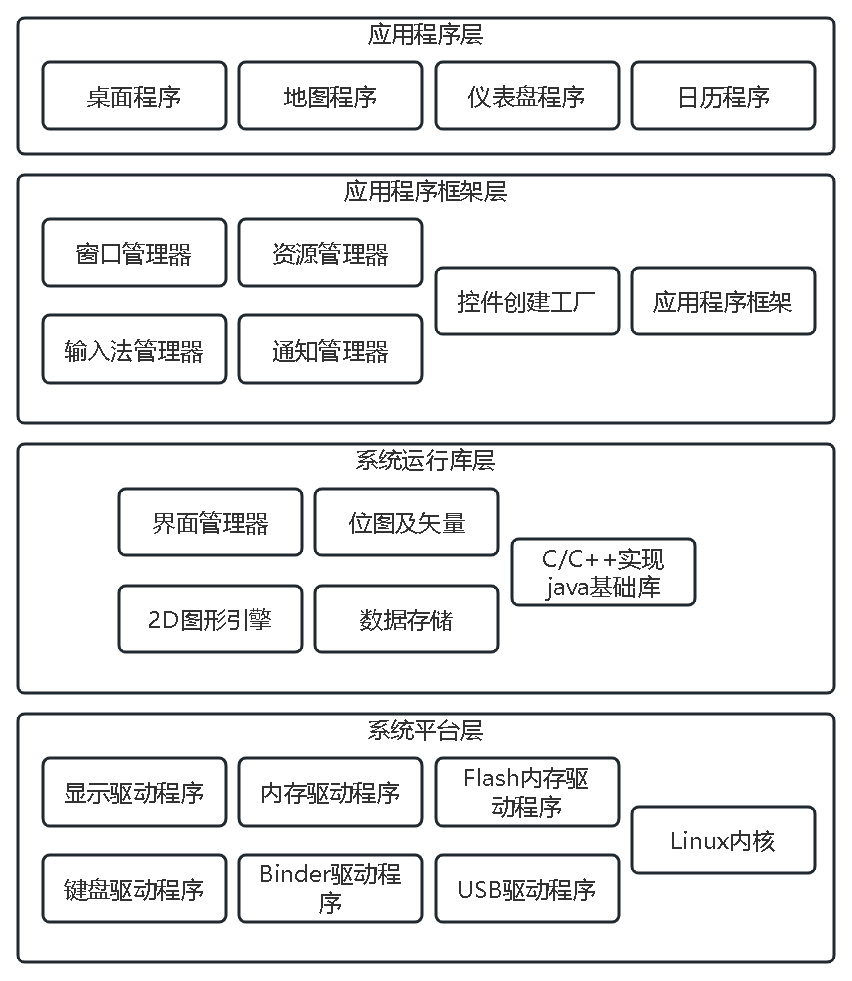
\includegraphics[width=0.5\textwidth]{cnd系统架构.pdf}
  \caption{cnd系统架构\cite{1016779798.nh}}
\end{figure}

高胜寒基于国产图形处理器设计了一套图形硬件抽象层\cite{高胜寒2019基于国产}。该方案对下可兼容国产化GPU硬件,对上可兼容图形API,且可支持多个操作系统。
\begin{figure}[H]
  \centering
  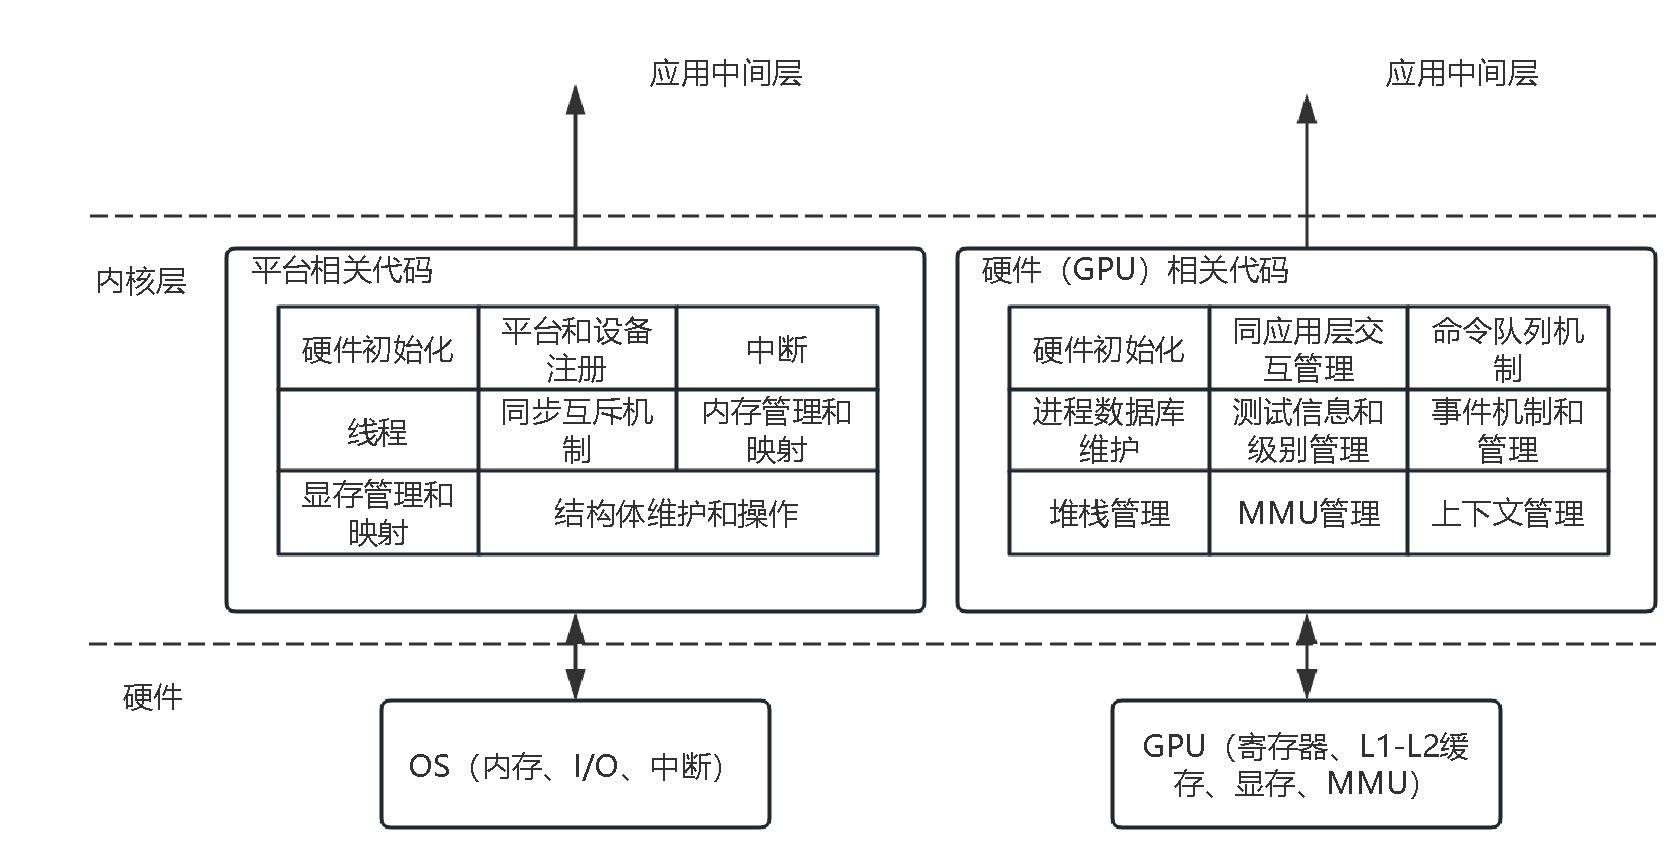
\includegraphics[width=0.8\textwidth]{内核层模块示意图.pdf}
  \caption{内核层模块示意图\cite{高胜寒2019基于国产}}
\end{figure}

\section{本文主要工作}

本课题以在LoongArch架构上构建可运行的Android运行环境,并打通图形系统相关依赖,从而实现安卓上层应用可以调用运行龙芯LG110显卡实现图形加速的目的。
在对Android系统结构、源码以及图像系统进行分析的基础上,移植并实现了一套可以在龙芯3A5000和7A2000桥片(包含LG110显卡)上运行的安卓图形系统运行环境。
主要包括以下内容:
\begin{itemize}
  \item 学习分析Android系统的结构和图形系统的运行机制,为后续添加龙芯硬件支持打下基础
  \item 基于安卓5.10内核,实现了基于龙芯LG110显卡的内核驱动模块,包括设计IOCTL命令码以及多版本适配的方案。
  \item 完成安卓图形系统依赖的供应商库硬件混合渲染模块和图形缓存分配模块的实现
  \item 为龙芯安卓系统构建OpenGL ES支持,并根据目标硬件平台缺陷完成了系统定制方面的工作,以支持16k page\_size等特性
  \item 调试测试整个图形栈,搭建系统运行环境并打通显示通路。
\end{itemize}
%MARK:创新点依旧有待商榷。
本文的预期目标是能够在安卓平台下正确调用LG110显卡,并运行Android Native程序,在3A5000硬件平台下运行启动安卓系统并进入开机动画,并成功通过相关
程序的测试和验证。

\section{本文的组织架构}
本文第一章是绪论部分,介绍研究背景和意义,国内外研究现状,并对全文的组织结构进行阐述。

第二章围绕课题介绍了AOSP开源安卓项目,介绍了AOSP构建系统以及Native程序运行的支持库,以及以介绍AOSP源码树为切入点介绍本课题所涉及的部分。
介绍了安卓图形系统的各个组件,包括低级别组件以及高级别组件等。随后介绍了GPU的软件栈,包括核模块、mesa、libdrm以及DRM等。

第三章从图形系统关键服务SurfaceFlinger分析开始,分析了如何将安卓图形系统运行在LoongArch架构下的龙芯显卡这一硬件平台上。分析了安卓的兼容性需求,
驱动接口的需求,架构上的差异等,明确设计方案。随后从内核模块的实现,硬件混合渲染模块和图形缓存分配模块三个方面介绍了现有工作,最后介绍了
构建龙芯OpenGL ES支持以及安卓系统镜像定制方面的内容

第四章是系统测试,分别介绍了现有的测试平台以及测试内容,包括DRM接口测试以及谷歌官方提供的测试套件。

第五章对论文的工作内容作了总结,分析了所构建系统的优势与不足,并对课题的未来研究方向做出了一些展望和建议。

